%
% Main document
% ===========================================================================
% This is part of the document "Project documentation template".
% Authors: brd3, kaa1
% Version: 1.2
%

%---------------------------------------------------------------------------
\documentclass[
	a4paper,				% paper format
	10pt,					% fontsize
	twoside,				% double-sided
	openright,				% begin new chapter on right side
	notitlepage,			% use no standard title page
	parskip=half,			% set paragraph skip to half of a line
]{scrreprt}					% KOMA-script report
%---------------------------------------------------------------------------

\raggedbottom
\KOMAoptions{cleardoublepage=plain}			% Add header and footer on blank pages


% Load Standard Packages:
%---------------------------------------------------------------------------
\usepackage[standard-baselineskips]{cmbright}

\usepackage[ngerman]{babel}										% german hyphenation
\usepackage[utf8x]{inputenc}  									% Unix/Linux - load extended character set
%\usepackage[ansinew]{inputenc}  								% Windows - load extended character set (ISO 8859-1)
\usepackage[T1]{fontenc}										% hyphenation of words with ä,ö and ü
\usepackage{textcomp}											% additional symbols
\usepackage{ae}													% better resolution of Type1-Fonts 
\usepackage{fancyhdr}											% simple manipulation of header and footer 
\usepackage{etoolbox}											% color manipulation of header and footer
\usepackage{graphicx}                      						% integration of images
\usepackage{float}												% floating objects
\usepackage{caption}											% for captions of figures and tables
\usepackage{booktabs}											% package for nicer tables
\usepackage{tocvsec2}											% provides means of controlling the sectional numbering
\usepackage{tabularx}
\usepackage{minted}
\usepackage{setspace}\setstretch{1.3} % for custom spacing



%---------------------------------------------------------------------------

% Load Math Packages
%---------------------------------------------------------------------------
\usepackage{amsmath}                    	   	% various features to facilitate writing math formulas
\usepackage{amsthm}                       	 	% enhanced version of latex's newtheorem
\usepackage{amsfonts}                      		% set of miscellaneous TeX fonts that augment the standard CM
\usepackage{amssymb}							% mathematical special characters
\usepackage{exscale}							% mathematical size corresponds to textsize
%---------------------------------------------------------------------------

% Package to facilitate placement of boxes at absolute positions
%---------------------------------------------------------------------------
\usepackage[absolute]{textpos}
\setlength{\TPHorizModule}{1mm}
\setlength{\TPVertModule}{1mm}
%---------------------------------------------------------------------------					
			
% Definition of Colors
%---------------------------------------------------------------------------
\RequirePackage{color}                          % Color (not xcolor!)
\definecolor{linkblue}{rgb}{0,0,0.8}            % Standard
\definecolor{darkblue}{rgb}{0,0.08,0.45}        % Dark blue
\definecolor{bfhgrey}{rgb}{0.41,0.49,0.57}      % BFH grey
%\definecolor{linkcolor}{rgb}{0,0,0.8}     		% Blue for the web- and cd-version!
\definecolor{linkcolor}{rgb}{0,0,0}        		% Black for the print-version!
%---------------------------------------------------------------------------

% Hyperref Package (Create links in a pdf)
%---------------------------------------------------------------------------
\usepackage[
	pdftex,ngerman,bookmarks,plainpages=false,pdfpagelabels,
	backref = {false},					  % No index backreference
	colorlinks = {true},                  % Color links in a PDF
	hypertexnames = {true},               % no failures "same page(i)"
	bookmarksopen = {true},               % opens the bar on the left side
	bookmarksopenlevel = {0},             % depth of opened bookmarks
	pdftitle = {Template für Bachelor Thesis},	   	% PDF-property TODO
	pdfauthor = {brd3},        					  % PDF-property TODO
	pdfsubject = {LaTeX Template},        % PDF-property TODO
	linkcolor = {linkcolor},              % Color of Links
	citecolor = {linkcolor},              % Color of Cite-Links
	urlcolor = {linkcolor},               % Color of URLs
]{hyperref}
%---------------------------------------------------------------------------

% Set up page dimension
%---------------------------------------------------------------------------
\usepackage{geometry}
\geometry{
	a4paper,
	left=28mm,
	right=15mm,
	top=30mm,
	headheight=20mm,
	headsep=10mm,
	textheight=242mm,
	footskip=15mm
}


\newcommand{\code}[1]{\texttt{#1}}

%---------------------------------------------------------------------------

% Makeindex Package
%---------------------------------------------------------------------------
\usepackage{makeidx}                         	% To produce index
\makeindex                                    	% Index-Initialisation
%---------------------------------------------------------------------------

% Glossary Package
%---------------------------------------------------------------------------
%\usepackage[nonumberlist]{glossaries}
\usepackage[acronym, toc]{glossaries}
\makenoidxglossaries

\newacronym{iot}{IoT}{Internet of Things}

%\newacronym{mqtt}{MQTT}{Message Queuing Telemetry Transport}

\newglossaryentry{mqtt}
{
    name=MQTT,
    description={Netzwerkprotokoll für IoT Anwenungen}
}







% Demo
\newglossaryentry{maths}
{
    name=mathematics,
    description={Mathematics is what mathematicians do}
}

\newacronym{lcm}{LCM}{Least Common Multiple}
%---------------------------------------------------------------------------

% Intro:
%---------------------------------------------------------------------------
\begin{document}                              	% Start Document
\settocdepth{section}							% Set depth of toc
\pagenumbering{roman}														
%---------------------------------------------------------------------------

\providecommand{\titel}{MQTT Device Description}					% Titel der Arbeit aus Datei titel.tex lesen
\providecommand{\versionnumber}{0.1}			%  Hier die aktuelle Versionsnummer eingeben
\providecommand{\versiondate}{23.08.2015}		%  Hier das Datum der aktuellen Version eingeben				% Versionsnummer und -datum aus Datei version.tex lesen

% Set up header and footer
%---------------------------------------------------------------------------
\makeatletter
\patchcmd{\@fancyhead}{\rlap}{\color{bfhgrey}\rlap}{}{}		% new color of header
\patchcmd{\@fancyfoot}{\rlap}{\color{bfhgrey}\rlap}{}{}		% new color of footer
\makeatother

\fancyhf{}																		% clean all fields
\fancypagestyle{plain}{												% new definition of plain style	
	\fancyfoot[OR,EL]{\footnotesize \thepage} 	% footer right part --> page number
	\fancyfoot[OL,ER]{\footnotesize \titel, Version \versionnumber, \versiondate}	% footer even page left part 
}

\renewcommand{\chaptermark}[1]{\markboth{\thechapter.  #1}{}}
\renewcommand{\headrulewidth}{0pt}				% no header stripline
\renewcommand{\footrulewidth}{0pt} 				% no bottom stripline

\pagestyle{plain}
%---------------------------------------------------------------------------


% Title Page and Abstract
%---------------------------------------------------------------------------
%%
% Project documentation template
% ===========================================================================
% This is part of the document "Project documentation template".
% Authors: brd3, kaa1
%

\begin{titlepage}



% BFH-Logo absolute placed at (28,12) on A4 
% Actually not a realy satisfactory solution but working.
%---------------------------------------------------------------------------
\setlength{\unitlength}{1mm}
\begin{textblock}{20}[0,0](28,12)
	
\includegraphics[scale=1.0]{bilder/BFH_Logo_B.png}
\end{textblock}
\color{black}

% Institution / Titel / Untertitel / Autoren / Experten:
%---------------------------------------------------------------------------
\begin{flushleft}

\vspace*{21mm}

\fontsize{26pt}{28pt}\selectfont 
\titel 				\\							% Titel aus der Datei vorspann/titel.tex lesen
\vspace{2mm}

\fontsize{16pt}{20pt}\selectfont\vspace{0.3em}
Beschreibung von vernetzten Geräten mit MQTT  			\\
\vspace{5mm}

\fontsize{10pt}{12pt}\selectfont
\textbf{Bachelorthesis} \\
\vspace{3mm}



\begin{textblock}{150}(28,225)
\fontsize{10pt}{17pt}\selectfont
\begin{tabbing}
xxxxxxxxxxxxxxx\=xxxxxxxxxxxxxxxxxxxxxxxxxxxxxxxxxxxxxxxxxxxxxxx \kill
Studiengang:	\> Informatik	\\
Autor:		    \> Adrian Bärtschi		\\
Betreuer:		\> Prof. Dr. Ing. Reto E. Koenig		\\
Experte:		\> Dr. Federico Flueckiger				\\
Datum:			\> \versiondate					\\		% aus Datei vorspann/version.tex lesen
\end{tabbing}

\end{textblock}
\end{flushleft}

\begin{textblock}{150}(28,280)
\noindent 
\color{bfhgrey}\fontsize{9pt}{10pt}\selectfont
Berner Fachhochschule | Haute école spécialisée bernoise | Bern University of Applied Sciences
\color{black}\selectfont
\end{textblock}



\end{titlepage}

%
% ===========================================================================
% EOF
%		% activate for Titelseite ohne Bild
%
% Project documentation template
% ===========================================================================
% This is part of the document "Project documentation template".
% Authors: brd3, kaa1
%

\begin{titlepage}

\begin{singlespacing}


% BFH-Logo absolute placed at (28,12) on A4 and picture (16:9 or 15cm x 8.5cm)
% Actually not a realy satisfactory solution but working.
%---------------------------------------------------------------------------
\setlength{\unitlength}{1mm}
\begin{textblock}{20}[0,0](28,12)
	
\includegraphics[scale=1.0]{bilder/BFH_Logo_B.png}
\end{textblock}

\begin{textblock}{154}(28,48)
	\begin{picture}(150,2)
		\put(0,0){\color{bfhgrey}\rule{150mm}{2mm}}
	\end{picture}
\end{textblock}

\begin{textblock}{154}[0,0](28,50)
	
\includegraphics[scale=1.0]{bilder/platzhalter.jpg}			% Titelbild definieren
\end{textblock}

\begin{textblock}{154}(28,135)
	\begin{picture}(150,2)
		\put(0,0){\color{bfhgrey}\rule{150mm}{2mm}}
	\end{picture}
\end{textblock}
\color{black}

% Institution / Titel / Untertitel / Autoren / Experten:
%---------------------------------------------------------------------------
\begin{flushleft}

\vspace*{115mm}

\fontsize{26pt}{28pt}\selectfont 
\titel 				\\							% Titel aus der Datei vorspann/titel.tex lesen
\vspace{2mm}

\fontsize{16pt}{20pt}\selectfont\vspace{0.3em}
Hier steht ein Untertitel 			\\							% Untertitel eingeben
\vspace{5mm}

\fontsize{10pt}{12pt}\selectfont
\textbf{Bachelorthesis} \\
\vspace{3mm}



\begin{textblock}{150}(28,225)
\fontsize{10pt}{17pt}\selectfont
\begin{tabbing}
xxxxxxxxxxxxxxx\=xxxxxxxxxxxxxxxxxxxxxxxxxxxxxxxxxxxxxxxxxxxxxxx \kill
Studiengang:	\> Informatik	\\
Autor:		    \> Adrian Bärtschi		\\
Betreuer:		\> Prof. Dr. Ing. Reto E. Koenig		\\
Experte:		\> Dr. Federico Flueckiger				\\
Datum:			\> \versiondate					\\		% aus Datei vorspann/version.tex lesen
\end{tabbing}

\end{textblock}
\end{flushleft}

\begin{textblock}{150}(28,280)
\noindent 
\color{bfhgrey}\fontsize{9pt}{10pt}\selectfont
Berner Fachhochschule | Haute école spécialisée bernoise | Bern University of Applied Sciences
\color{black}\selectfont
\end{textblock}

\end{singlespacing}


\end{titlepage}

%
% ===========================================================================
% EOF
%			% activate for Titelseite mit Bild
% Versionenkontrolle :
% -----------------------------------------------

\begin{textblock}{180}(15,150)
\color{black}
\begin{huge}
Versionen
\end{huge}


\setstretch{1.0} % Version Table kompakter
\vspace{10mm}

\fontsize{10pt}{18pt}\selectfont
\begin{tabbing}
xxxxxxxxxxx\=xxxxxxxxxxxxxxx\=xxxxxxxxxxxxxx\=xxxxxxxxxxxxxxxxxxxxxxxxxxxxxxxxxxxxxxxxxxxxxxx \kill
Version	\> Datum	\> Status		\> Bemerkungen		\\
0.1	\> 23.08.2015	\> Entwurf		\> Dokument erstellt	\\	
0.2	\> 05.10.2015	\> Entwurf		\> Einleitung, Bestehenden Ansätze \\	
0.3	\> 27.10.2015	\> Entwurf		\> Kozept\\	
0.4	\> 15.11.2015	\> Entwurf		\> Projektmanagement	\\	
0.5	\> 10.01.2016	\> Entwurf		\> Anforderungen, Verifikation \\	
0.6	\> 11.01.2016	\> Entwurf		\> Umsetzung\\
0.7	\> 18.01.2016	\> Entwurf		\> Fazit, Review, Abrunden des Dokuments\\
1.0	\> 21.01.2016	\> Final		    \> Abgabe\\
\end{tabbing}

\end{textblock}


\setstretch{1.3} % Rest des Dokuments wieder 1.3
\cleardoubleemptypage
\setcounter{page}{1}
\cleardoublepage
\phantomsection 
\addcontentsline{toc}{chapter}{Management Summary}
\chapter{Management Summary}
\label{chap:managementSummary}

\color{black}

- Was ist das Ziel der Thesis \\
- Kurzbeschrieb des Themas \\
- Was wurde gemacht, erreicht \\
\cleardoubleemptypage
%---------------------------------------------------------------------------

% Table of contents
%---------------------------------------------------------------------------
\tableofcontents
\cleardoublepage
%---------------------------------------------------------------------------

% Main part:
%---------------------------------------------------------------------------
\pagenumbering{arabic}

\chapter{Einleitung}
\label{chap:einleitung}


\acrfull{iot} ist momentan einer der grossen Trends in der Informatik und demensprechend wagen immer mehr Unternehmen erste Versuche in diesem Umfeld. Da es für die Umsetzung von IoT Systemen noch keine grossen Erfahrungswerte und 'Best-Practices' gibt, ist die Entwicklung von Prototypen ein geeignetets Hilfsmittel. Für diesem Zweck gibt es bereits mehrere Produkte auf dem Markt, unter anderen das Tinkerforge System. Die darin enthaltenen Bausteine (Sensoren, Displays, LEDS, Buttons, etc.) können auf einfache Weise ohne Werkzeug zusammengesteckt werden. 
Um die einzelnen Komponenten anzusprechen, zum Beipspiel für die Abgrage eines Sensorwerts, muss ein Programm erstellt werden, welches mithilfe der bereitgestellten Libraries die Komponenten initialisiert und ansteuert.

Beim Bau von Prototypen sind schnelle Ergegebenisse und häufiges Anpassen des Systems wichtige Aspekte. Wenn nach dem Zusammensetzen der Hardware Komponenten das System selbständig die Daten in einer Schnittstelle zur Verfügung stellen würde, könnte das dem Entwickler der eigentlich Anwendung viel Aufwand ersparen. Er müsste sich nicht mehr um die Initialisierung der Komponenten und das Auslesen und Aggregieren der Daten kümmern.

Stattdessen kann er auf einfache Weise auf die Daten zugreifen seine Applikation losgelöst davon entwerfen und implementieren. 



\chapter{Einleitung v2}
Bei Anwendungen, die im aufstrebenden Bereich von \acrfull{iot} angesiedelt sind, spielt das Netwerkprotokoll \Gls{mqtt} eine wichtige Rolle. Damit lassen sich beliebige Nutzdaten an verschiedenen Empfänger versenden. Der einfache und leichtgewichtige Aufbau des Protokolls hat viele Vorteile bei eingeschränkten Systemen, bringt aber auch gewisse Schwierigkeiten mit sich.

Netzwerkteilnehmer, welche eine Nachricht empfangen, müssen deren Syntax und Semantik kennen um die Daten sinnvoll auswerten zu können. Wie diese Beschreibung der Daten strukturiert werden und den Emfängern der Daten zur Verfügung gestellt wird, ist derzeit ein unglöstes Problem. Die meisten Systeme, die \Gls{mqtt} bereits einsetzen, liefern die Dokumentation in einen separaten Dokument. \\
Bei häufigen Änderungen der Datenstruktur hat dies einen grossen Aufwand für das Nachführen der Dokumentation zur Folge.

Anwendugen, welche selbst mit einem Dienst oder Gerät via \Gls{mqtt} kommunizieren wollen, brauchen eine Beschreibung der zur Verfügung stehenden Operationen. Beispielsweise muss eine vernetze Glühbirne wie man sie ein- und ausschalten kann und welche Informationen ausgelesen werden können.

\chapter{Einleitung v3}
Bei Systemen im \acrfull{iot} Umfeld sind sehr viele und auch unterschiedliche Geräte in einen Netzwerk miteindander verbunden. 
Für diese IoT - Machine-To-Machine Kommunikation werden andere Netzwerkprotokolle eingesetzt als im 'klassischen' Internet. Dies ist nötig, weil die Geräte stark eingeschränkte Resourcen haben und die Netzwerke geringe Bandbreiten aufweisen.

MQTT ist ein Protokoll, welches die Anforderungen für IoT Systeme erfüllen soll. Beim Entwurf des Protokolls wurde auf Einfachheit und Leichtgewichtigkeit grossen Wert gelegt. Mit MQTT ist es möglich, beliebige Daten in beliebiger Codierung zu versenden. Dies bietet den Entwicklern der Systeme grosse Freiheiten. \\
Es ist aber ersichtlich, dass die fehlende Struktur und Beschreibung der Daten gewisse Schwierigkeiten mit sich bringen kann. Eine Anwendung, welche Daten per MQTT erhält, muss wissen wie diese vom Absender codiert wurden und was sie bedeuten.

Um diese Information vom Anbieter der Daten resp. des Diestes oder Geräts den Entwicklern einer Anwedung zur Verfügung zu stellen, werden zurzeit Beschreibungen in Dokumentenform verwendet. Diese sogenannte out-out-band Dokumentation ist aber aufwändig in der Nachführung und bekanntegabe von Änderungen. Auch ist es schwierig die Struktur der Daten einheitlich und klar zu erklären.

Ziel dieser Thesis ist es, dass Geräte welche ihre Daten per MQTT versenden, die Möglichkeit erhalten, sich selbst inkusive ihrer Daten und Möglichkeiten zur Interkation zu beschreiben. Dies soll so getan werden, dass die Beschreibung für Mensch und Maschine les- und verstehbar ist, die Eigenschaften der eingeschränkten Geräte und Netze berücksichtig wird und der MQTT Standard weiterhin eigehalten wird.


\chapter{Related Work}

\section{Tinkerforge MQTT Proxy}
% www.tinkerforge.com/en/doc/Software/Brick_MQTT_Proxy.html

Python Script, Doku Homepage

Eigene Impl. Java

\section{CoAP?}

\section{Eclipse Vorto}
% https://www.eclipse.org/vorto/index.html

\section{OMA LWM2M - Leshan}
% https://eclipse.org/leshan/

\section{Konzept aus der nicht-IoT Welt}
SOAP-WSDL, REST, etc.
HATEOAS

MQTT REST
http://dejanglozic.com/2014/05/06/rest-and-mqtt-yin-and-yang-of-micro-service-apis/


%\chapter{Anleitungen}
\label{chap:anleitungen}

Die nachfolgende Tabelle zeigt einige der wichtigsten Pakete\index{Paket}, die in der \LaTeX{} Vorlage verwendet werden.

\begin{table}[H]
	\centering
		\begin{tabular}{p{0.13\textwidth} p{0.75\textwidth}} \toprule
			\textbf{Paket} & \textbf{Funktion} \\ \midrule
			\texttt{cmbright}\index{cmbright} & Serifenlose Schriftart 'Computer Modern Bright' welche die Textcodierungen\index{Textcodierungen} OT1, T1 und TS1 unterstützt, sowie die mathematischen Zeichen wie auch die AMS Symbole \\ \midrule
			\texttt{ae} & Sorgt für besser aufgelöste Schriften in PDF Dateien \\ \midrule
			\texttt{fancyhdr}\index{fancyhdr} & Einfache Anpassung der Kopf- und Fusszeilen \\ \midrule
			\texttt{graphicx}\index{graphicx} & Einbindung von Grafiken in \LaTeX{} dokumente \\ \midrule
			\texttt{booktabs}\index{booktabs} & Schönere Darstellung von Tabellen \\ \midrule
			\texttt{textpos}\index{textpos} & Vereinfachte absolute Positionierung von Boxen auf der Seite \\ \midrule
			\texttt{hyperref}\index{hyperref} & Paket zum Erstellen von Links in PDF Dateien \\ \midrule
			\texttt{geometry}\index{geometry} & Vereinfachte und verbesserte Anpassung des Standard-Satzspiegels \\ \midrule
			\texttt{makeidx}\index{makeidx} & Einfache Indexerstellung (siehe Kapitel \ref{sec:anleitungen_index})\\ \midrule
			\texttt{glossaries}\index{glossaries} & Erstellen von Glossaren (siehe Kapitel \ref{sec:anleitungen_glossar}) \\ \bottomrule
		\end{tabular}
	\caption{Pakete}
	\label{tab:pakete}
\end{table}


\section{Stichwortverzeichnisse}
\label{sec:anleitungen_index}

\LaTeX{} ist in der Grundausstattung nicht fähig ein \gls{StwVrz} \index{Stichwortverzeichnis} zu erstellen. Diese können in \LaTeX{} mit dem \texttt{makeidx} Paket und dem \texttt{makeindex}\index{makeindex} Programm erstellt werden. Die folgende Seite enthält eine ausführliche Erklärung wie das Paket funktioniert und dessen Anwendung:

\begin{center}
	\url{http://de.wikibooks.org/wiki/LaTeX-W%C3%B6rterbuch:_makeindex}
\end{center}

Grob zusammengefasst sind für ein Stichwortverzeichnis folgenden Punkte nötig:

\begin{itemize}
	\item Einbinden des Paketes \texttt{makeidx}
	\item Durch den \texttt{\textbackslash makeindex} Befehl die Erstellung initialisieren
	\item Im Text laufend Wörter indexieren mit dem Befehl \texttt{\textbackslash index\{\}}
	\item Beim ersten Durchlauf der Dokumenterstellung wird das Verzeichnis erstellt und die mit \texttt{\textbackslash index\{\}} markierten Begriffe in der \texttt{.idx}-Datei gespeichert
	\item Beim zweiten Durchlauf wird die \texttt{.idx}-Datei sortiert, formatiert und als \texttt{.ind}-Datei abgespeichert, wobei \LaTeX{} nun die \texttt{.ind}-Datei in das Dokument einfügt
\end{itemize}

\section{Glossar}
\label{sec:anleitungen_glossar}

Ein Glossar\index{Glossar} kann in \LaTeX{} ebenfalls mit dem \texttt{makeindex} Programm und dem \texttt{glossaries} Paket erstellt werden. Die folgende Auflistung zeigt das Vorgehen um ein Glossar zu erzeugen:

\begin{itemize}
	\item Einbinden des \texttt{glossaries} Pakets
	\item Falls es als sinnvoll erachtet wird, kann eine eigene Datenbank mit Glossareinträgen erstellt werden. In dieser Vorlage wird mit einer solchen Datenbank gearbeitet, welche im Ordner \texttt{datenbanken} abgelegt ist. Einträge aus der Datenbank werden nur in das Verzeichnis geschrieben, falls das Wort im Text auch wirklich vermerkt ist.
	\item Durch den \texttt{\textbackslash makeglossaries} Befehl wird die Erstellung initialisiert
	\item Neue Einträge können mit dem Befehl \\ \texttt{\textbackslash newglossaryentry\{<ABKÜRZUNG>\}\{name=\{<NAME>\},description=\{<BESCHRIEB>\}\}} \\ erstellt werden
	\item Im Text laufend Wörter referenzieren mit dem Befehl \texttt{\textbackslash gls\{<ABKÜRZUNG>\}}
	\item Ähnlich wie bei der Erstellung des Index, wird das Verzeichnis erst beim zweiten Durchlauf in das Dokument eingebunden
\end{itemize}

Damit das Ganze überhaupt funktioniert, muss als Nachbearbeitung des Dokuments das Glossar mit \texttt{makeindex} erstellt werden. Dazu ist folgender Code in der Kommandozeile auszuführen:

\begin{center}
	\texttt{makeindex -s template.ist -t template.glg -o template.gls template.glo}
\end{center}

Bei den meisten \LaTeX -Editoren kann dies als Nachbearbeitungsschritt angegeben werden. Die nachfolgende Erklärung ist für das Programm TeXnicCenter. Unter dem Menupunkt \glqq Ausgabe\grqq{} -> \glqq Ausgabeprofile definieren\grqq{} (kurz: alt + F7) ist unter dem Register \glqq Nachbearbeitung\grqq{} das in Bild \ref{fig:nachbearbeitung} dargestellte Fenster zu finden. Anschliessend gilt es, einen neuen Eintrag einzufügen, wobei eine Anwendung wie auch ein Argument anzugeben ist. Die Anwendung ist in der MiKTeX Installation zu finden (\texttt{..\textbackslash MiKTeX X.X\textbackslash miktex\textbackslash bin\textbackslash makeindex.exe}). Als Argument ist die folgende Zeile eizutragen:

\begin{center}
	\texttt{-s \string"\%tm.ist\string" -t \string"\%tm.glg\string" -o \string"\%tm.gls\string" \string"\%tm.glo\string" }
\end{center}

\begin{figure}[H]
	\centering
		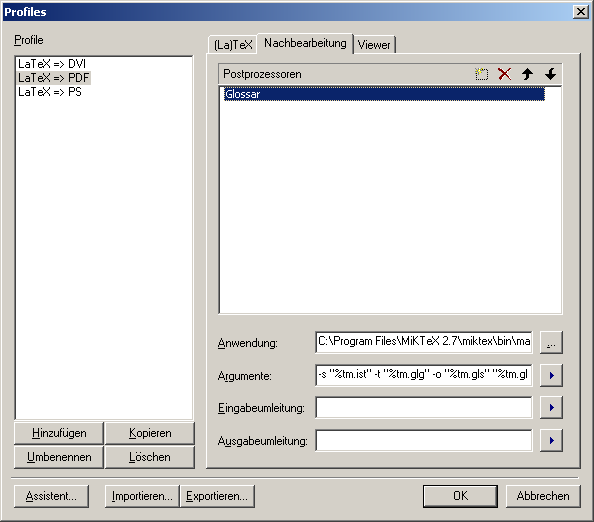
\includegraphics[scale=0.7]{bilder/profiles_glossar.png}
	\caption{Nachbearbeitung}
	\label{fig:nachbearbeitung}
\end{figure}


\section{Bibliographie}
\label{sec:anleitungen_bibliographie}

Zur Erstellung einer Bibliographie\index{Bibliographie} wird auf \gls{BibTeX} zurückgegriffen. Im Ordner \texttt{datenbanken} befindet sich eine \texttt{.bib}-Datei mit diversen Datenbankeinträgen. Wie diese Einträge zu erstellen sind, kann aus diversen Quellen im Internet oder in Büchern entnommen werden. Die Einträge in der Datenbank werden nur dann in das Verzeichnis des Dokuments geschrieben, wenn die Quelle auch wirklich im Text zitiert wurde.

Unter den folgenden Adressen sind weitere Erläuterungen zum Erstellen der Datenbank und deren Verwendung zu finden:
\begin{itemize}
	\item \url{http://en.wikipedia.org/wiki/BibTeX}
	\item \url{http://www.bibtex.org/de/}
\end{itemize}
\chapter{Projektmanagement}
\label{chap:projectmanagement}

\section{Organisation}

\begin{table}[H]
\begin{tabularx}{\textwidth}{|l|l|X|}

 \hline \rowcolor{lightgray}
 {\bf Name } & {\bf Rolle } & {\bf Aufgaben} \\  \hline
  \parbox[t]{5cm}{\textbf{Prof. Dr. Ing. Reto E. König} \\ \textit{Berner Fachhochschule}}  &   Betreuer  &
  Hauptansprechsperson für Studierenden, verantwortlich für den Ablauf der Thesis. Beurteilung aufgrund von Aufgabenstellung und abgegebenen Artefakten.   \\
 \hline
  \parbox[t]{5cm}{\textbf{Dr. Federico Flueckiger} \\ \textit{Eidg.  Finanzdepartement}} &   Experte     &
  Beurteilung aufgrund der Aufgabenstellung und abgelieferten Artefakten sowie mindestends ein bis zwei Sitzungen mit dem Studierenden. \\ 
\hline
 \textbf{Adrian Bärtschi}                &   Studierender   &     
 Selbständiges Projektmanagement während der Thesis. Setzt die Aufgaben gemäss Aufgabenstellung und Vorgaben des Betreuers um. Organisiert Kommunikation mit dem Betreuer und Experten.   \\
 \hline


\end{tabularx}
\caption{Involvierte Personen und deren Aufgaben}
\end{table}


\section{Ziele}
Die Arbeit umfasst gemäss Aufgabenstellung folgende Ziele:
\begin{itemize}
    \item Definition einer Beschreibungssprache für vernetzte Geräte.
    \item Die Beschreibung muss von Menschen und Computern interpretiert werden können.
    \item Die Beschreibung muss die Eingabe- und Ausgabeparameter der Geräte beeinhalten.
    \item Die Beschreibung soll möglichst die aktuelle MQTT Spezifikation (3.1.1) nicht verletzen.
\end{itemize}

\section{Meilensteine}

Die Aufgabenstellung wurde in Meilensteine aufgeteilt, um eine grobe Planung zu erhalten.

\begin{table}[H]
\begin{tabularx}{\textwidth}{|l|X|}

 \hline \rowcolor{lightgray}
 {\bf Datum } & {\bf Meilenstein } \\  \hline
 
 25.09.2015  &   Initialisierung, Vorgehen geklärt      \\ \hline
 01.10.2015  &   Ziele definiert      \\ \hline
 15.10.2015  &   Einfacher Prototyp erstellt, Konzept der Lösung skizziert     \\ \hline
 30.11.2015  &   Spezifikation Device Description festgelegt     \\ \hline
 15.12.2015  &   Implementation Demo Applikation abgeschlossen     \\ \hline
 18.01.2016  &   Dokumentation inhaltlich abgeschlossen      \\ \hline
 21.01.2016  &   Dokumentation fertiggestellt, Präsentation vorbereitet     \\ \hline
 
\end{tabularx}
\caption{Meilensteine der Thesis}
\end{table}


\section{Ressourcen}

Die gesamte Thesis umfasst gemäss Modulplan der BFH einen Arbeitsaufwand von 360 Stunden. Dies beinhaltet die Konzeption und Umsetzung der Lösung, Abprachen mit Betreuer und Experte, das Erstellen der Dokumentation und die Vorbereitung der Präsentationen für den Finaltag und die Verteidigung.

Es sind keine Kosten für Softwarelizenzen oder andere Ressourcen angefallen.


\section{Aufwände}
Nachfolgend ist der Gesamtaufand von 360 Stunden der Arbeit auf einzelen Tasks aufgeteilt. Ausserdem werden bei grösseren Differenzen zwischen geplanten und geleisteten Stunden die Gründe dafür angegeben.

\begin{table}[H]
\begin{tabularx}{\textwidth}{|l|r|r|X|}

 \hline \rowcolor{lightgray}
 {\bf Task } & { \bf Geplant [h] } & {\bf Ist [h] }  & {\bf Bemerkungen } \\  \hline
 \textbf{Projektmanagement}         &      &       &   \\ \hline
 Kickoff, Initialisierung           &   8  &   8   &   \\ \hline
 Ziele definieren                   &   6  &   8   &   \\ \hline
 Planung Tasks                      &   8  &  10   &   \\ \hline
 Meetings Betreuer                  &  10  &  12   &   \\ \hline
 Meetings Experte                   &   4  &   2   &  Nur ein Meeting nötig \\ \hline
     &      &       &   \\ \hline
 \textbf{Umsetzung}                 &      &       &   \\ \hline
 MQTT Device Description Library    &  32  &  28   &   \\ \hline
 Tinkerforge Prototyp Java          &  50  &  52   &   \\ \hline
 Webapplikation Device Browser      &  40  &  42   &   \\ \hline
     &      &       &   \\ \hline
 \textbf{Dokumentation}             &      &       &   \\ \hline
 Setup                              &   4  &   8   &  Probleme mit Online Latex Umgebung \\ \hline
 Projektmanagement                  &  16  &  20   &   \\ \hline
 Einleitung, bestehende Umsetzungen &  32  &  30   &   \\ \hline
 Konzept und Anforderungen          &  16  &  18   &   \\ \hline
 Spezifikation Device Description   &  16  &  12   &   \\ \hline
 Umsetzung                          &  32  &  36   &   \\ \hline
 Fazit                              &   8  &   8   &   \\ \hline
 Finalisierung                      &  24  &  22   &   \\ \hline
     &      &       &   \\ \hline
 \textbf{Präsentation}              &      &       &   \\ \hline
 Poster                             &   8  &   8   &   \\ \hline
 Book Seite                         &   8  &  11   &  Mehrere Reviews, Korrekturen nötig\\ \hline
 Präsentation Finaltag              &  24  &  18   &   \\ \hline
 Präsentation Verteidigung          &  14  &  10   &   \\ \hline
     &      &       &   \\ \hline
     &      &       &   \\ \hline
 \textbf{Total}                     & \textbf{360}  &  \textbf{363}     &   \\ \hline

\end{tabularx}
\caption{Planung der Tasks und Auswertung der geleisteten Stunden}
\end{table}


\section{Termine / Abgabefristen}
\begin{table}[H]
\begin{tabularx}{\textwidth}{|l|X|}

 \hline \rowcolor{lightgray}
 {\bf Datum } & {\bf Beschreibung } \\  \hline
 04.01.2016   & Abgabe elektronische Form des Posters  \\ \hline
 11.01.2016   & Erfassung und Freigabe der Book Seite  \\ \hline
 21.01.2016   & Abgabe Dokumentation an Betreuer, Experte und BFH  \\ \hline
 22.01.2016   & Finaltag Bern, Präsentation und Ausstellung \newline
                Abgabe Dokumentation gedruckt und Source Code an Sekretariat BFH  \\ \hline
 01.02.2016   & Verteidigung \\ \hline

\end{tabularx}
\caption{Termine und Fristen}
\end{table}

\section{Ablage}
Diese Dokumentation sowie sämltlicher Source Code sind auf dem Github Repository unter \\ \url{https://github.com/barta3/ch.bfh.bti7321thesis.mqttSemantics} verfügbar.

\section{Reflektion}

Dieser Abschnitt blickt auf das Vorgehen während der Thesis zurück und beschreibt kurz die wichtigsten Eindrücke.

Da die Aufgabenstellung relativ offen formuliert ist, war es zu Beginn der Arbeit schwierig sich vorzustellen wie die Lösung aussehen soll und was sie alles beinhaltet. In dieser Phase haben vor allen die regelmässigen Besprechungen mit Reto König geholfen, um Ideen zu diskutieren und jeweils die nächsten Schritte zu planen.

Aufgrund der geringen Verbreitung und Bekanntheit des MQTT Protokolls sind keine etablierten Lösungen vorhanden, von deren Erfahrungen man profitieren konnte. Dies bot jedoch auch eine grosse Freiheit bei der Gestaltung und Umsetzung der eigenen Lösung.

Beim Entwurf der Device Description und der Umsetzung hat sich gezeigt, dass sich ein iteratives Vorgehen   gut eignet. Mit der frühen Entwicklung von Prototypen und ständiger Verbesserung und Anpassung konnte die Aufgabenstellung gut in kleinere Pakete aufgeteilt werden.

Da die eingesetzten Devices von Tinkerforge viele verschiedene Interaktionsmöglichkeiten bieten, konnten nicht alle Funktionen mit der Device Description abgebildet werden. Bei Devices, welche einen spezifischeren Einsatzzweck haben, sollten dann die Device Descriptions auch enstsprechend kompakter werden.


Für die Erarbeitung der Dokumentation wurde LaTeX verwendet, basierend auf der Vorlage der BFH. Dies hat sich nach anfänglichen Schwierigkeiten bei der Installation als gute Entscheidung erwiesen. Dank der vordefinierten Formatierung konnte ich mich auf die das Erstellen der Inhalte konzentrieren. Ausserden eignete sich diese Dokumentationsform gut für das eingesetzte Versionskontrollsystem (Git).

Je technischer die Dokumentation wurde, desto umständlicher wurde es, die Inhalte verständlich in Deutscher Sprache zu formulieren. Rückblickend wäre es ev. besser gewesen, das Dokument in Englisch zu verfassen, vor allem um die technischen Begriffe einheitlicher verwenden zu können.

\chapter{Technologie}
\label{chap:technologie}


\section{State-of-the-art}
Die verschiedenen Hersteller von MQTT Anwendungen entwickeln jeweils ihre eigenen Ansätze, um die Daten zu strukturieren. 

\subsection{Tinkerforge MQTT Proxy}

\subsection{IBM Internet of Things Foundation}

IBM stellt den Service 'IBM IoT Foundation' zur Verfügung, mit dem vernetzte Geräte verwaltet werden können. Als Kommunikationsprotokoll wird MQTT eingesetzt. Die Platform verwendet folgende konzeptioneielle Ideen:
\begin{itemize}
    \item Organizations: Eindeutige Identifikation der Kunden der Platform
	\item Devices: Beliebiges vernetztes Gerät. Versendet Events und reagiert auf Commands.
	\item Applications: Anwendung, welche mit den Daten der Devices interagiert.
	\item Events: Daten, welche von den Devices an die Platform gesendet werden
	\item Commands: Applications können mittels Commands mit den Devices kommunizieren.
\end{itemize}

Events müssen an ein definiertes Topic nach folgendem Schema gesendet werden: \\
\code{iot-2/evt/\textbf{event\_id}/fmt/\textbf{format\_string}}

Beispiel: \code{iot-2/evt/temperature\_outdoor/fmt/json}

Eine Anwendung, welche Events empfangen möchte, muss sich auf ein Topic in der Form \\
\code{iot-2/type/\textbf{device\_type}/id/\textbf{device\_id}/evt/\textbf{event\_id}/fmt/\textbf{format\_string}} registrieren.
Die Teile \code{device\_type}, \code{device\_id}, \code{event\_id} und \code{format\_string} des Topics können auch mit dem Wildcard Charakter '\code{+}' ersetzt werden, um jeweils alle Events der Komponenten zu erhalten. 

Beispiel: \code{iot-2/type/temp/id/+/evt/temperature\_outdoor/fmt/+}

Um einen Command zu erzeugen, sendet eine Anwendung eine MQTT Message mit Topic gemäss folgenden Schema:
\code{iot-2/type/device\_type/id/device\_id/cmd/command\_id/fmt/format\_string}

Beispiel: \code{iot-2/type/temp/id/sensor1/cmd/setInterval/fmt/json}

Das Device \code{sensor1} würde damit eine Message auf Topic \code{iot-2/cmd/setInterval/fmt/json} erhalten.


Grundsätzlich unterstützt IBM IoT Foundation ein beliebiges Payload Format. Es wird jedoch empfohlem, JSON zu verwenden. Um alle Funktionen der Platform zu nutzen, müssen die JSON Dokumente zusätzlich nach den Vorgaben von IBM strukturiert sein.

\begin{listing}[H]
\begin{minted}[frame=single,
               framesep=3mm,
%               linenos=true,
               xleftmargin=21pt,
               tabsize=4]{json}
{
  "d": {
    "host": "IBM700-R9E683D",
    "mem": 54.9,
    "network": {
      "up": 1.22,
      "down": 0.55
    },
    "cpu": 1.3,
  }
}
\end{minted}
\caption{JSON Beispiel im IBM IoTF Payload Format}
\label{json-example}
\end{listing}
\begin{minted}{json}
\end{minted}



\section{MQTT}
Aus Proj2 übernehmen

\section{Tinkerforge}
Beschreibung,
%Hinweis auf www.tinkerforge.com/en/doc/Software/Brick_MQTT_Proxy.html

\section{DFDL}
Aus Proj2 übernehmen



% \section{CoAP?}

% \section{Eclipse Vorto}
% https://www.eclipse.org/vorto/index.html

% \section{OMA LWM2M - Leshan}
% https://eclipse.org/leshan/

\section{Konzept aus der nicht-IoT Welt}
SOAP-WSDL, REST, etc.
HATEOAS

\chapter{Konzept}
\label{chap:konzept}


\chapter{Umsetzung}
\label{chap:umsetzung}

Die Umsetzung hatte drei Module als Ergebnis.

\section{MQTT Device Description Library}
Um die Integration von Devices und das Erstellen von Device Description zu vereinfachen, wird eine Java Library entwickelt. Damit ist es möglich, Anwendugen für IoT Gateways in Java zu entwickeln. Zusammen mit der 

Die Library übernimmt folgende Aufgaben:
\begin{itemize}
\item Handling der MQTT Verbindung zum Broker
\item Versenden von Event- Command-, und State Informationen mittels MQTT Messages
\item Einheitliche Abbildung der Devices und Topics
\item Hilfsklassen zur Erstellung der Device Descriptions
\end{itemize}

Die Parameter der Library (MQTT Broker, Application ID, etc.) müssen vom Aufrufer der Library konfiguriert werden können.


\subsection{Klassendiagramm}

\begin{figure}[H]
	\centering
		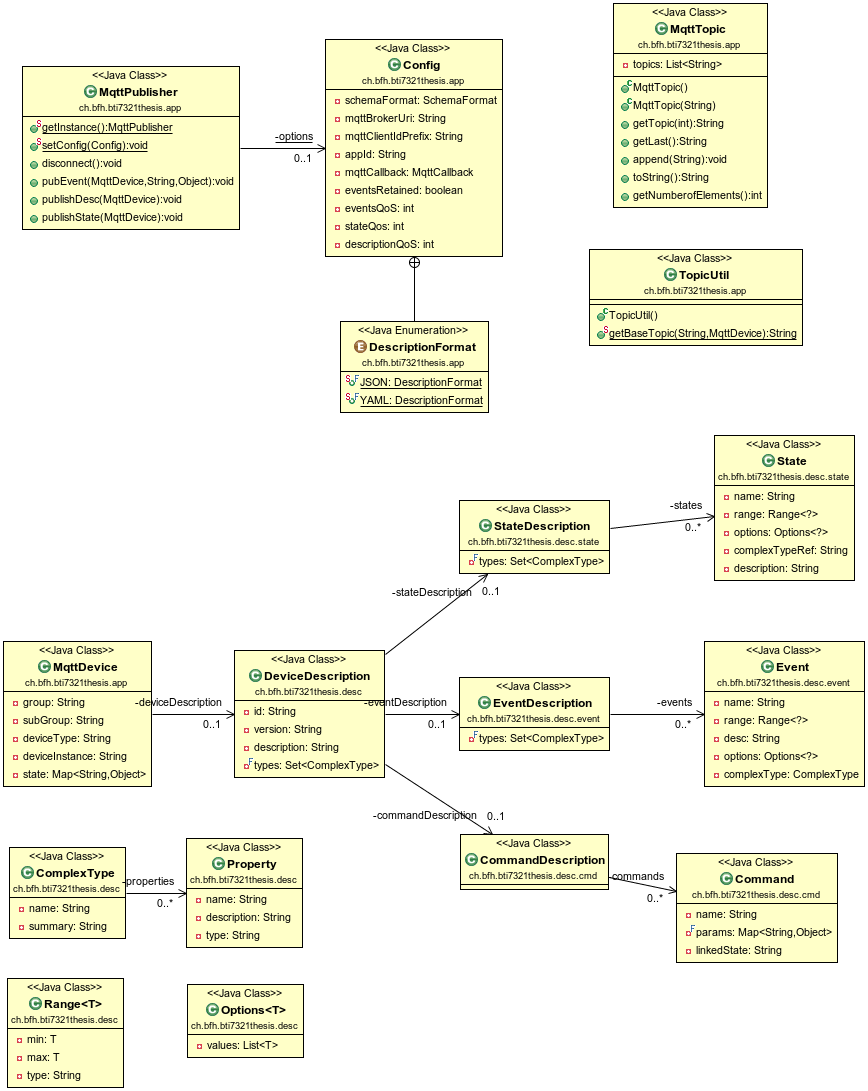
\includegraphics[width=1.0\textwidth]{diag/Lib_class_overview.png}
	\caption{Klassendiagramm MQTT Device Description Library}
\end{figure}

\begin{table}[H]
\begin{tabularx}{\textwidth}{|l|X|}

 \hline \rowcolor{lightgray}
 {\bf Klasse } & {\bf Zweck } \\  \hline
 
 MqttPublisher & Hauptklasse der Library. wird verwendet für das versenden der MQTT Nachrichten. \\ \hline

 Config & Wird verwendet, um bei der Initialsierung von MqttPublisher die Konfiguration abzugeben \\ \hline
 
 DescriptionFormat & Enum mit der Angaben zu den möglichen Formaten der Device Description.\\ \hline
 
 MqttTopic & Hilfsklasse die Abbildung von MQTT Topics.\\ \hline
 
 TopicUtil & Hilfsklasse für die Erstelltung von MQTT Topics.\\ \hline
 
 MqttDevice & Klasse für die Abbildung von Devices. \\ \hline
 
 DeviceDescription & Enhält alle Attribute der DeviceDescription.  \\ \hline
 
\end{tabularx}
\caption{Beschreibung der Klassen}
\end{table}

\subsection{Verwendung}
Die Device Description Library muss als erstes im eigenen Java Projekt eingebunden werden. Dies kann manuell mit der generierten .jar Datei (ch.bfh.barta3.mqttdevicedescription-1.0.0.jar) oder als Dependency Deklaration eines Maven Projektes getan werden.

\begin{listing}[H]
\begin{minted}[frame=single,
               framesep=3mm,
               linenos=false,
               xleftmargin=21pt,
               tabsize=4]{xml}
<dependency>
	<groupId>ch.bfh.barta3.mqttdevicedescription</groupId>
	<artifactId>ch.bfh.barta3.mqttdevicedescription</artifactId>
	<version>1.0.0</version>
</dependency>
\end{minted}
\caption{Maven Dependency MQTT Device Description Library}
\end{listing}

Als erstes muss die Konfiguration erstellt und an die Klasse \code{MqttPublisher} übergeben werden. Danach muss das Device inklusive Description erstellt werden. Sobald dies erfolgt ist, ist kann die Library beginnen, Daten zu versenden und reagiert auf empfangene Commands.

\begin{listing}[H]
\begin{minted}[frame=single,
               framesep=3mm,
               linenos=false,
               xleftmargin=21pt,
               tabsize=4]{java}

...

// Define Config
Config options = new Config();
options.setMqttBrokerUri("tcp://iot.eclipse.org:1883");
options.setAppId("myApp");
options.setMqttCallback(new MyCallbackHandler());
MqttPublisher.setConfig(options);
	
// Create Device and Description	
MqttDevice device = new MqttDevice("Bern", "Wankdorf", "Temp", "t1");	
device.setDeviceDescription(new DeviceDescription("test", "1.0"));
...

// Start publishing
MqttPublisher.getInstance().publishDesc(device);
MqttPublisher.getInstance().pubEvent(device, "event", "22");

...

\end{minted}
\caption{Einfaches Beipsiel für die Verwendung der Library}
\end{listing}

\textbf{Konfiguration} \\
Über das \code{Config} Objekt wird dierLibrary konfiguriert. Folgende Parameter können gesetzt werden:



\begin{table}[H]
\begin{tabularx}{\textwidth}{|l|X|}

 \hline \rowcolor{lightgray}
 {\bf Name } & {\bf Beschreibung }  \\  \hline
 
 mqttBrokerUri & Pflichtfeld. URI des MQTT Brokers (inkl. Protokoll und Port) \newline Beispiel: tcp://iot.eclipse.org:1883 \\ \hline
 
 mqttClientIdPrefix & Prefix für die ClientIds der MQTT Connections. Es werden zwei Connections aufgebaus. Für das Publishing eine mit ClientId {[mqttClientIdPrefix]}\_pub und eine Connection für das Empfangen von Messages mit ClientId {[mqttClientIdPrefix]}\_sub \newline Falls kein Wert angegeben wird, wird eine zufälliges Prefix generiert. \\ \hline
 
 appId & Pflichtfeld. Identifikation der Applikation. \\ \hline
 
 mqttCallback & Pflichtfeld. Implementation des Interfaces org.eclipse.paho.client.mqttv3.MqttCallback. Wird wird aufgerufen, wenn die Devices einen Command erhalten. \\ \hline
 eventsRetained &  true / false. Gibt an, ob die Event Messages mit Retained Flag versendet werden sollen. \newline Standard: true \\ \hline
 
 descriptionFormat & Format der Device Description. Mögliche Werte: YAML, JSON. \newline Standard: YAML \\ \hline
 
 eventsQoS & Gibt an, mit welcher \gls{qos} die Event Messages versendet werden sollen (0, 1, 2). \newline Standard: 1 \\ \hline
 
 stateQos & Gibt an, mit welcher \gls{qos} die State Messages versendet werden sollen (0, 1, 2). \newline Standard: 1 \\ \hline
 
 descriptionQoS & Gibt an, mit welcher \gls{qos} die Description Messages versendet werden sollen (0, 1, 2). \newline Standard: 1 \\ \hline
 
\end{tabularx}
\caption{Konfigurationsoptionen der Library}
\end{table}



\subsection{Verwendete Komponenten} {

Für die Umsetzung der MQTT Device Description Library wurden folgende Komponenten integriert:

\begin{table}[H]
\begin{tabularx}{\textwidth}{|l|X|}

 \hline \rowcolor{lightgray}
 {\bf Komponente } & {\bf Beschreibung }  \\  \hline
 
 Eclipse Paho & MQTT Client Implementation. \newline \url{http://www.eclipse.org/paho} \\ \hline

 Jackson JSON Processor & JSON Serialisierung und Parsing \newline \url{http://wiki.fasterxml.com/JacksonHome} \\ \hline
 
 Jackson Modul YAML & Erweiterung der Jackson Library für das YAML Datenformat \newline \url{https://github.com/FasterXML/jackson-dataformat-yaml} \\ \hline
 
\end{tabularx}
\caption{Externe Komponenten}
\end{table}


\section{Device Browser}
Mit der entwickelten Webapplikation lassen sich die Device Descriptions übersichtlich darstellen. Die Applikation ist als reine Clientanwendung in Javascript umgesetzt.
Die Anwenung zeigt die auf einem Broker publizierten Devices in einer Liste an. Zu einem Device kann der Benutzer sich die Device Description im Klartext anzeigen lassen. Die Device Description wird interpretiert und unterteilt in die verschiedenen Bereiche werden die Attribute angezeigt.

\begin{figure}[H]
	\centering
		\frame{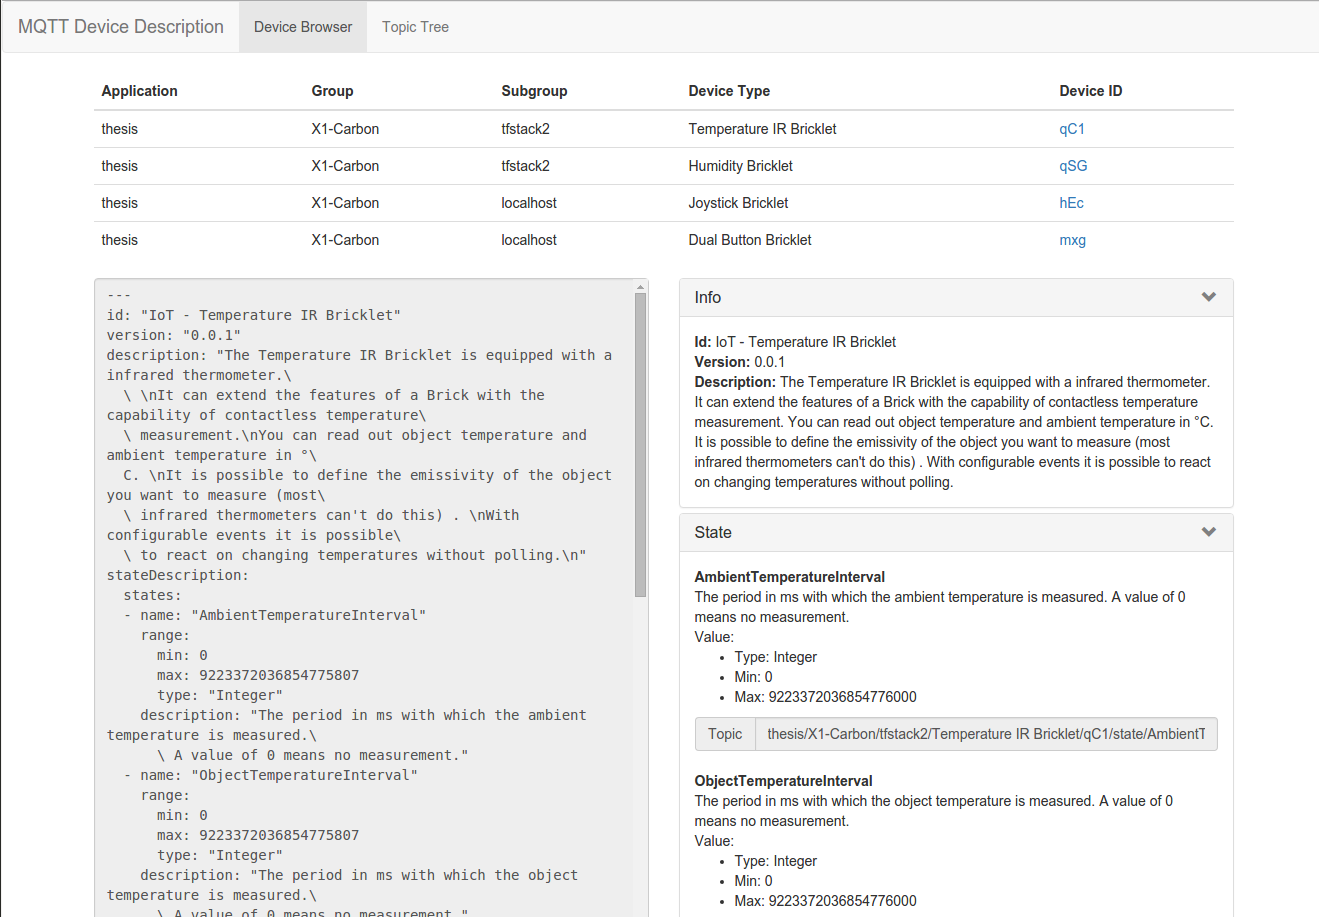
\includegraphics[width=1.0\textwidth]{bilder/device_browser_1.png}}
	\caption{Screenshot Device Browser}
\end{figure}

\textbf{Bereich State} \\
Die State Objekte werden mit Beschreibung und den Typangaben anzezeigt. Zudem wird das Topic ausgegeben, auf welchem die entsprechenden State Informationen publiziert wurden.

\newpage
\textbf{Bereich Events}

\begin{figure}[H]
	\centering
        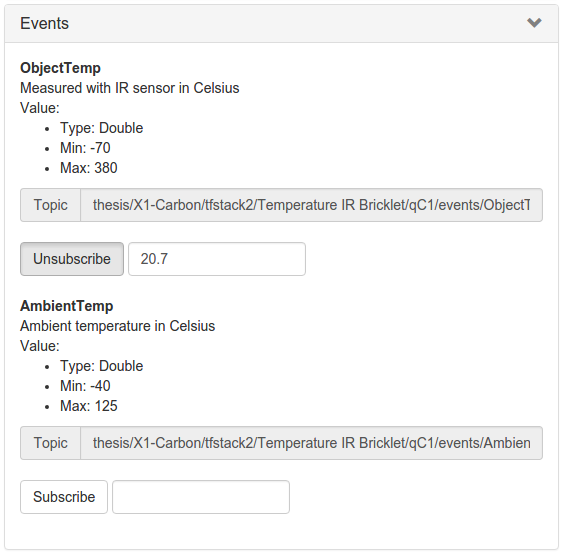
\includegraphics[width=0.7\linewidth]{bilder/device_browser_events.png} 
    \caption{Device Browser Event Darstellung}
\end{figure}

Die Event Informationen werden mit Name, Beschreibung und Angaben zum Typ angezeigt. Pro Events wird das Topic ausgegeben. Mit dem betötigen der Schaltfläche 'Subscribe' verbindet sich die Webaplikation auf das Topic des Events und zeigt die empfangenen Daten im Textfeld an. Mit einem Erneuten Klick auf die Schaltfläche wird die Verbindung beendet.

\newpage
\textbf{Bereich Commands}

\begin{figure}[H]
	\centering
        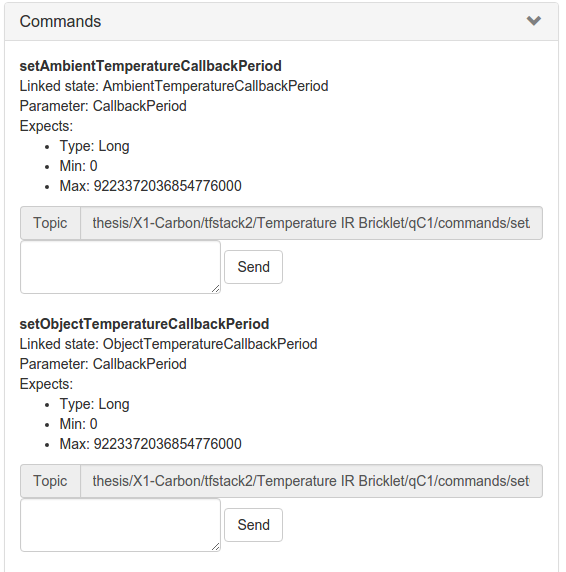
\includegraphics[width=0.7\linewidth]{bilder/device_browser_commands.png} 
    \caption{Device Browser Command Darstellung}
\end{figure}

Für die Command Objekte der Device Description werden nebst Name, Beschreibung und den erwarteten Typinforamtionen auch das Topic angezeigt, auf welches der Command gesendet werden muss. Es steht ein Eingabefeld zur Verfügung, in welchem der Payload der MQTT Message eingegeben werden kann. Mit dem Betätigen der Schaltfläche 'Send' wird der Command an das selektierte Device gesendet.


\textbf{Bereich Complex Types} \\
\begin{figure}[H]
	\centering
        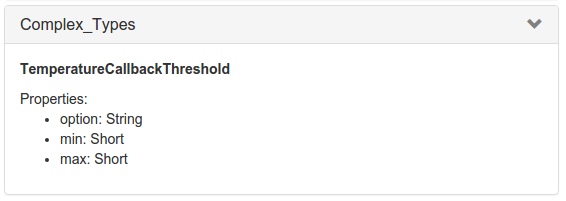
\includegraphics[width=0.7\linewidth]{bilder/device_browser_comptypes.png} 
    \caption{Device Browser Complex Type Darstellung}
\end{figure}

Falls das Schema Complex Types beinhaltet, werden diese hier aufgelistet. Für jeden Complex Type wird der Name und eine Liste der Properties (Attribute) aufgeführt.

\textbf{Topic Tree} \\

Als zweiter Teil der Webapplikation ist die Darstellung aller MQTT Topics des konfigurierten Brokers eingebunden. Dafür wurde die Applikation 'd3-MQTT-Topic-Tree' von Ben Hardill (\url{https://github.com/hardillb/d3-MQTT-Topic-Tree}) verwendet.

\begin{figure}[H]
	\centering
        \frame{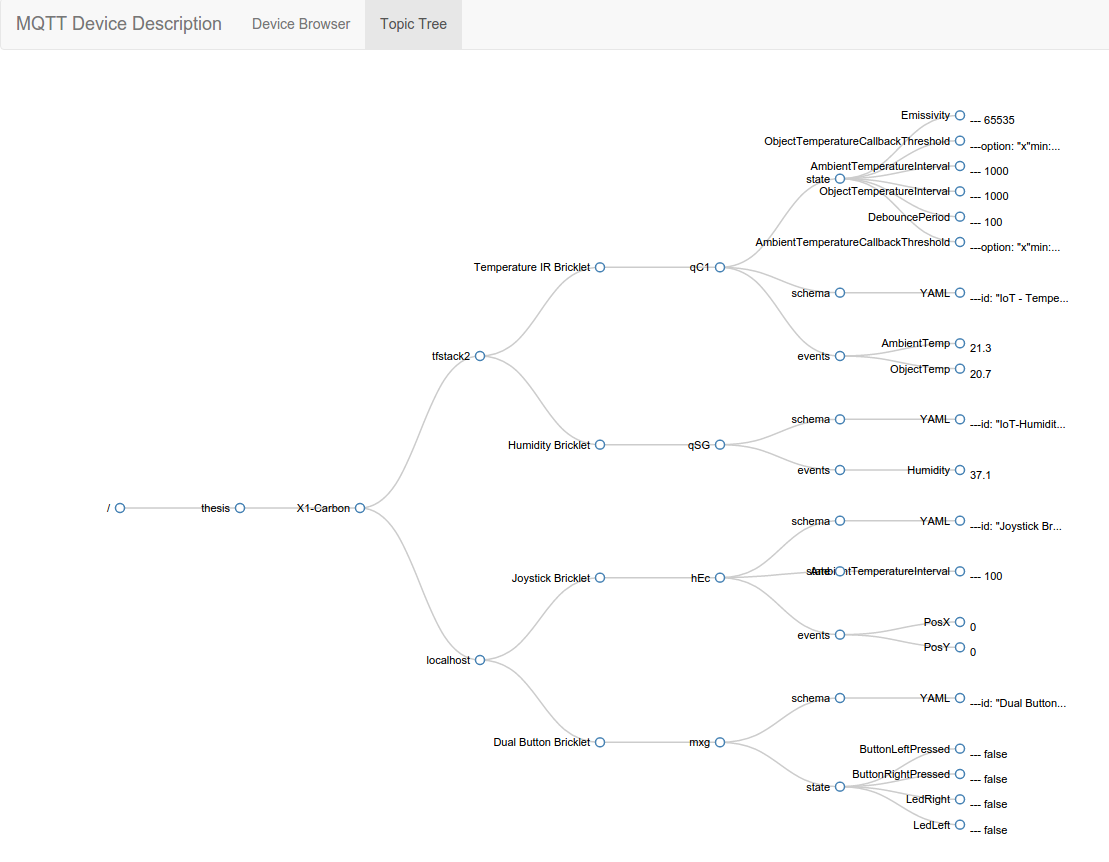
\includegraphics[width=1.0\linewidth]{bilder/topic_tree.png}}
    \caption{MQTT Topic Tree}
\end{figure}

Vor allen während der Entwicklung und dem Einbinden von neuen Devices hat sich diese Darstellung als sehr hilfreich erwiesen.

\subsection{Installation und Konfiguration}
Der MQTT Broker, auf den die Webapplikation zugreift, muss per Websockets erreichbar sein. Dafür eignet sich zum Beispiel der Mosquitto Broker. Während der Entwicklung der Applikationen wurde eine Mosquitto Installation mithilfe eines vorbereiteten Docker Images (\url{https://hub.docker.com/r/toke/mosquitto/}) durchgeführt und für sämtiche Testst verwendet.

Um die Webapplikation verwenden zu können, muss lediglich der Inhalt des Verzeichnisses \newline  \code{ch.bfh.bti7321thesis.schemabrowser} auf einen Webserver kopiert und die Datei \code{js/app/config.js} angepasst werden.

\begin{listing}[H]
\begin{minted}[frame=single,
               framesep=3mm,
               linenos=false,
               xleftmargin=21pt,
               tabsize=4]{js}

host = '46.101.165.125'; // hostname or IP address of broker
port = 9001;             // Websocket Port of broker
descFormat = 'YAML';     // YAML or JSON

\end{minted}
\caption{Beipiel Konfiguration Device Browser}
\end{listing}



%\newpage
\section{Anwendung Tinkerforge}

Um die MQTT Device Description Library an einem konkreten Beispiel zu testen, wurden verschiedene Bausteine des Tinkerforge Systems verwendet. Die Tinkerforge Bausteine (auch Bricklets genannt) haben den Vorteil, dass sie einfach zu verwenden sind und es bereits Libraries für die Kommunikation mit der Hardware gibt. Das Ziel der Anwendung war es, zu demonstrieren, dass es möglich ist konkrete Devices mit dem entwickelten Konzept resp. der Device Description Library zu beschreiben und eine Interaktion von ausserhalb per MQTT zu ermöglichen.

\begin{figure}[H]
	\centering
        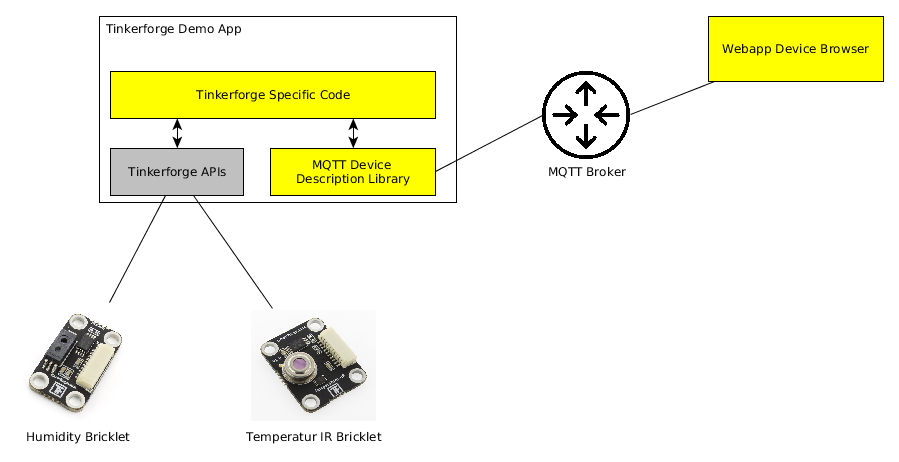
\includegraphics[width=1.0\linewidth]{diag/tf_arch.png}
    \caption{Aufbau der Tinkerforge Anwendung}
\end{figure}

\newpage
Folgende Sensoren resp. Aktoren wurden ausgewählt:

\def\imagetop#1{\vtop{\null\hbox{#1}}}

\begin{table}[H]
\begin{tabularx}{\textwidth}{|l|X|l|}

 \hline \rowcolor{lightgray}
 {\bf Komponente } & {\bf Beschreibung } & \textbf{Bild} \\  \hline
 
 Sensor Luftfeuchtigkeit & Misst die relative Luftfeuchtigkeit. 
 \newline Mehr Informationen: \newline \url{http://www.tinkerforge.com/en/doc/Hardware/Bricklets/Humidity.html} & 
 \imagetop{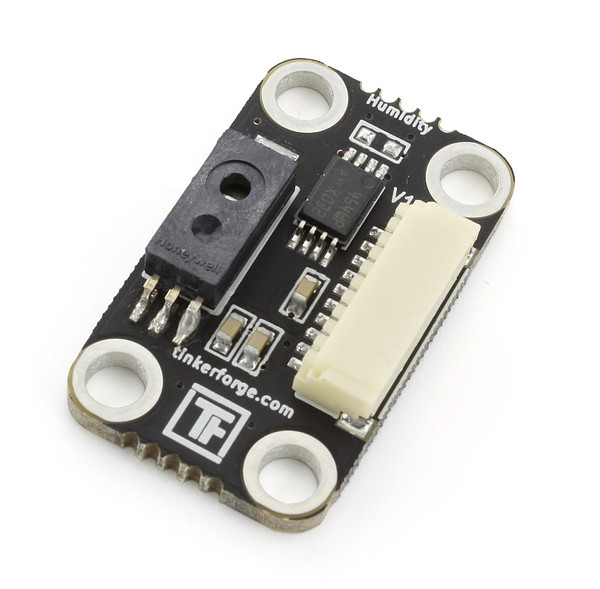
\includegraphics[width=0.4\linewidth]{bilder/bricklet_humidity.jpg}}    \\ \hline
 
 Sensor Temperatur Infrarot & Besteht einem Temperatursensor für die Umgebung und einem Infrarotsensor für die Messung der Objekttemperatur \newline 
 \newline Mehr Informationen: \newline \url{http://www.tinkerforge.com/en/doc/Hardware/Bricklets/Temperature_IR.html} & 
 \imagetop{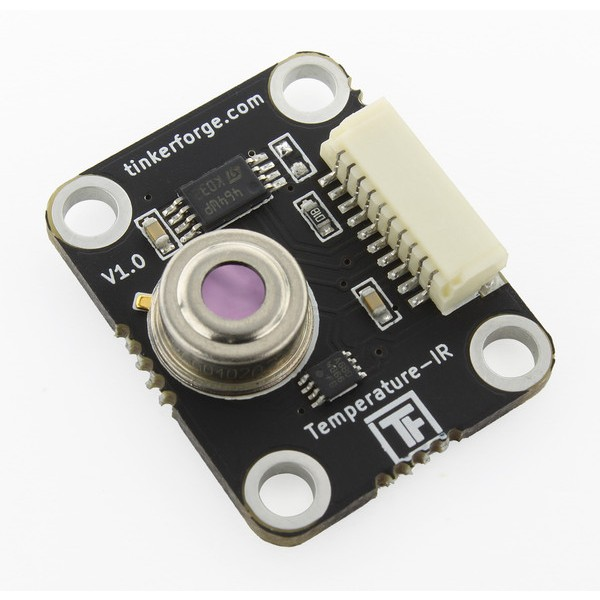
\includegraphics[width=0.4\linewidth]{bilder/bricklet_temperature_ir.jpg}}    \\ \hline
 
 Dual Button & Besteht aus zwei Buttons, welche je ein LED integriert haben. \newline 
 \newline Mehr Informationen: \newline \url{http://www.tinkerforge.com/en/doc/Hardware/Bricklets/Dual_Button.html} & 
 \imagetop{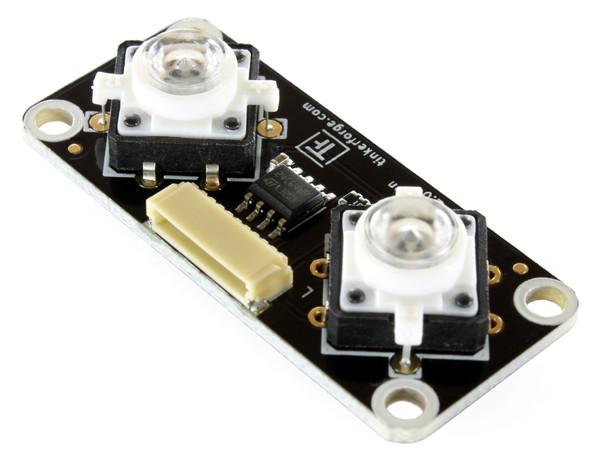
\includegraphics[width=0.4\linewidth]{bilder/bricklet_dual_button.jpg}}    \\ \hline

 \end{tabularx}
\caption{Verwendeten Tinkerforge Komponenten}
\end{table}

Quelle Bilder: \url{http://www.tinkerforge.com/en/doc/index.html}



\subsection{Klassendiagramm}

\begin{figure}[H]
	\centering
        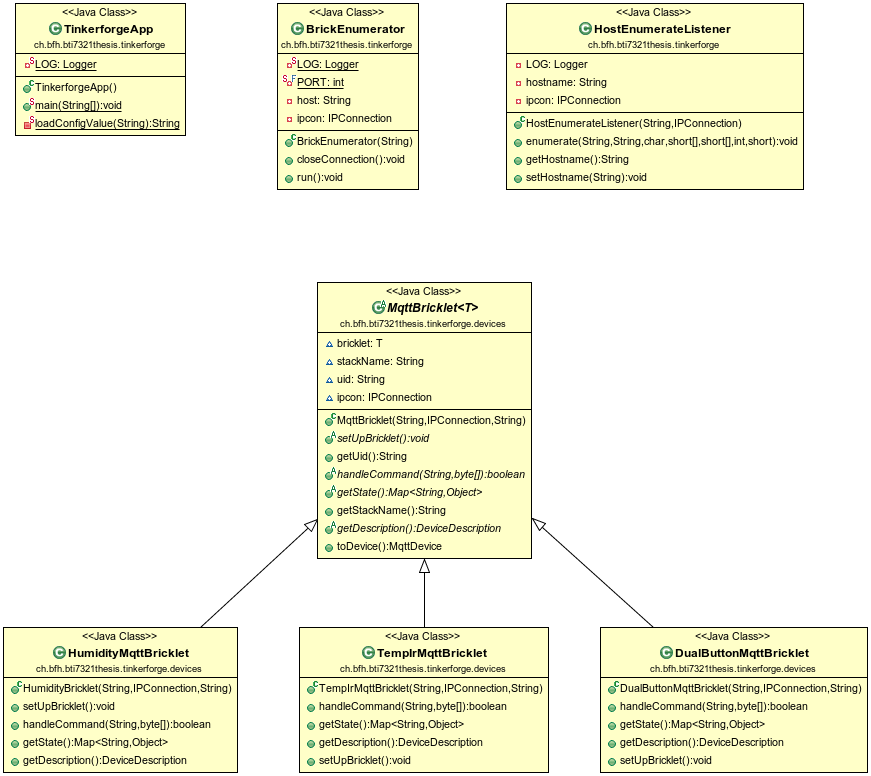
\includegraphics[width=1.0\linewidth]{diag/tf_overview_class.png}
    \caption{Klassendiagramm Tinkerforge Anwendung}
\end{figure}

\begin{table}[H]
\begin{tabularx}{\textwidth}{|l|X|}

 \hline \rowcolor{lightgray}
 {\bf Klasse } & {\bf Zweck } \\  \hline
 
 TinkerforgeApp & Start der Applikation, Einlesen der Konfiguration, Setup der MQTT Device Description Library. \\ \hline

 BrickEnumerator & Thread, welcher für jeden angegebenen Tinkerforge Stack die Devices (Bricklets) sucht. \\ \hline
 
 HostEnumerateListener & Epfängt die gefundenen Tinkerforge Devices und erstellt die entsprechenden \code{MqttBricklets} \\ \hline
 
 MqttBricklet &  Abstrakte Oberklasse für die konkreten Bricklet Implementationen. Definiert die abstrakten Methoden \code{setUpBricklet()}, \code{getState()}, \code{handleCommand(...)},  und \code{getDescription()}, welche von den Subklassen implementiert werden. \newline Mit der Methode \code{toDevice()} wird eine Instant der Klasse \code{MqttDevice} erzeugt wird, welche die Subklassen verwenden um z. Bsp. Events zu versenden. \\ \hline
 
 HumidityMqttBricklet &  Implementation für das Humidity Bricklet. \\ \hline
 
 TempIrMqttBricklet & Implementation für das Temperatur IR Bricklet. \\ \hline
 
 DualButtonMqttBricklet & Implementation für das Dual Button Bricklet.\\ \hline
 

\end{tabularx}
\caption{Beschreibung der wichtigsten Klassen}
\end{table}

\subsection{Device Descriptions}
Die Device Descriptions der drei behandelten Devices sind im Anhang TODO zu finden.


\chapter{Fazit}
\label{chap:schlussfolgerungen}

Es hat sich gezeigt, dass allgemein bei MQTT Anwendungen zwei Hauptschwierigkeiten auftreten. Zum einen gibt es keinen Mechanismus für die Angabe resp. das Finden (Discovery) der Topics auf dem Broker. Der zweite Punkt ist die fehlende Struktur der Message Payloads. 

Diese Grundprobleme treten auch beim Einsatz von MQTT für vernetzte Geräte in Erscheinung. Als Ergebnis der Arbeit ist ein Konzept entstanden, welches mithilfe einer definierten Topic Struktur und einem Schema für die Device Description einen möglichen Lösungsweg aufzeigt. Die Umsetzung eines Prototyps hat gezeigt, dass das Konzept grundsätzlich funktionstüchtig ist, jedoch noch Potenzial für Verbesserungen aufweist.

Als nächster Schritt wäre es interessant zu sehen, wie gut sich die entwickelten Ideen für einen konkreten Anwendungsfall aus der Praxis eignen und welche Anpassungen dafür ev. noch gemacht werden müssten.


Es gilt zu beachten, dass das Thema Internet of Things noch neu und stark in Bewegung ist. Ob sich ein einheitliches Konzept für die Beschreibung von Devices per MQTT einmal durchsetzen wird, ist momentan schwer abzuschätzen. Obwohl der Wunsch nach einheitlichen Schnittstellen vorhanden ist, gibt  es zurzeit wenig Anzeichen, dass sich ein Standard etablieren wird.
%---------------------------------------------------------------------------

% Selbständigkeitserklärung
%---------------------------------------------------------------------------
\cleardoublepage
\phantomsection 
\addcontentsline{toc}{chapter}{Selbständigkeitserklärung}
\chapter*{Selbständigkeitserklärung}
\label{chap:selbstaendigkeitserklaerung}

\vspace*{10mm} 

Ich bestätige mit meiner Unterschrift, dass ich meine vorliegende Bachelor-Thesis selbständig durchgeführt habe. Alle Informationsquellen (Fachliteratur, Besprechungen mit Fachleuten, usw.) und anderen Hilfsmittel, die wesentlich zu meiner Arbeit beigetragen haben, sind in meinem Arbeitsbericht im Anhang vollständig aufgeführt. Sämtliche Inhalte, die nicht von mir stammen, sind mit dem genauen Hinweis auf ihre Quelle gekennzeichnet
. 

\vspace{15mm}

\begin{tabbing}
xxxxxxxxxxxxxxxxxxxxxxxxx\=xxxxxxxxxxxxxxxxxxxxxxxxxxxxxx\=xxxxxxxxxxxxxxxxxxxxxxxxxxxxxx\kill
Ort, Datum:		\> Bern, \versiondate \\ \\ 
Namen Vornamen:	\> Bärtschi Adrian 	\\ \\ \\ \\ 
Unterschriften:	\> ......................................\> 
\end{tabbing}
%---------------------------------------------------------------------------

% Glossary, Acronyms
%---------------------------------------------------------------------------
\cleardoublepage
\phantomsection 
%\addcontentsline{toc}{chapter}{Glossar}
%\renewcommand{\glossaryname}{Glossar}
\printnoidxglossaries
\cleardoublepage
%\printglossary[type=\acronymtype]
%---------------------------------------------------------------------------

% Bibliography
%---------------------------------------------------------------------------
\cleardoublepage
\phantomsection 
\addcontentsline{toc}{chapter}{Literaturverzeichnis}
\bibliographystyle{IEEEtranS}
\bibliography{datenbanken/bibliography}{}
%---------------------------------------------------------------------------

% Listings
%---------------------------------------------------------------------------
\cleardoublepage
\phantomsection 
\addcontentsline{toc}{chapter}{Abbildungsverzeichnis}
\listoffigures
\cleardoublepage
\phantomsection 
\addcontentsline{toc}{chapter}{Tabellenverzeichnis}
\listoftables
%---------------------------------------------------------------------------

% Index
%---------------------------------------------------------------------------
\cleardoublepage
\phantomsection 
\addcontentsline{toc}{chapter}{Stichwortverzeichnis}
\renewcommand{\indexname}{Stichwortverzeichnis}
\printindex
%---------------------------------------------------------------------------

% Attachment:
%---------------------------------------------------------------------------
\appendix
\settocdepth{section}
\chapter{Beliebiger Anhang}
\label{chap:bel_anhang}

Phasellus eget velit massa, sed faucibus nisi. Etiam tincidunt libero viverra lorem bibendum ut rutrum nisi volutpat. Donec non quam vitae lacus egestas suscipit at eu nisi. Maecenas non orci risus, at egestas tellus. Vivamus quis est pretium mauris fermentum consectetur. Cras non dolor vitae nulla molestie facilisis. Aliquam euismod nisl eget risus pretium non suscipit nulla feugiat. Nam in tortor sapien. Nam lectus nibh, laoreet eu ultrices nec, consequat nec sem. Nulla leo turpis, suscipit in vulputate a, dapibus molestie quam. Vestibulum pretium, purus sed suscipit tempus, turpis purus fermentum diam, id cursus enim mi a tortor. Proin imperdiet varius pellentesque. Nam congue, enim sit amet iaculis venenatis, dui neque ornare purus, laoreet porttitor nunc justo vel velit. Suspendisse potenti. Nulla facilisi.
%---------------------------------------------------------------------------

%---------------------------------------------------------------------------
\end{document}